	\documentclass[]{report}
\usepackage{tikz}
\newcommand{\inputtikz}[2]{%  
	\scalebox{#1}{\input{#2}}  
}
\usepackage[french]{babel}
\usepackage[utf8x]{inputenc}
\usepackage{amsmath}
\usepackage{graphicx}
%\usepackage[colorinlistoftodos]{todonotestfa}
\usepackage{listings}
\usepackage{color}
\usepackage{amsmath}
\usepackage{amsfonts}
\usepackage{mathtools}
\usepackage{graphicx}
\usepackage{caption}
\definecolor{dkgreen}{rgb}{0,0.6,0}
\definecolor{gray}{rgb}{0.5,0.5,0.5}
\definecolor{mauve}{rgb}{0.58,0,0.82}
%opening

\lstset
{frame=tb,
	language=R,
	aboveskip=3mm,
	belowskip=3mm,
	showstringspaces=false,
	framexleftmargin=5mm,
	columns= fixed,
	numbers = left,
	basicstyle={\small\ttfamily},	
	numberstyle=\tiny\color{gray},
	keywordstyle=\color{blue},
	commentstyle=\color{dkgreen},
	stringstyle=\color{mauve},
	breaklines=true,
	breakatwhitespace=true,
	tabsize=3
}

\begin{document}
	
\begin{titlepage}
	
	\newcommand{\HRule}{\rule{\linewidth}{0.5mm}} 
	
	\center 
	
	\textsc{\LARGE Université de Technologie de Compiegne}\\[1.5cm]
	\textsc{\Large SY09}\\[0.5cm] 
	\textsc{\large Data Mining}\\[0.5cm]
		
	\HRule \\[0.4cm]
	{ \huge \bfseries Premier Rendu}\\[0.4cm] 
	\HRule \\[1.5cm]
		
	\begin{minipage}{0.4\textwidth}
		\begin{flushleft} \large
			Oumaima \textsc{Talouka} 
		\end{flushleft}
	\end{minipage}
	~
	\begin{minipage}{0.4\textwidth}
		\begin{flushright} \large
			Zineb \textsc{SLAM} 
		\end{flushright}
	\end{minipage}\\[2cm]

	{\large \today}\\[2cm] 

	
\includegraphics[width=40mm]{Figures/utc.jpg}\\ % 

	\vfill
	
\end{titlepage}



\begin{abstract}
Dans ce rapport du TP1 de l'UV SY09 nous allons expliquer notre démarches dans l'analyse des données en expliquant les résultats obtenus. Ce TP est compose de 2 parties. La première partie a pour objectif de se familiariser avec les méthodes de traitement et de visualisation de données sur R. La deuxième partie traite de l'Analyse en composantes principales (ACP). Nous allons travailler avec 3 dataset notes de SY02, Crabs et Pima qu'on va d'abord analyser et décrire avant d'y réaliser l'ACP en seconde partie. Pour les graphes obtenus nous avons utilises la librairie ggplot2 qui offre un grand nombre de fonctionnalité Le code R sera fourni en annexe.

\end{abstract}

\tableofcontents

\chapter{ Statistique descriptive}

\section{Notes SY02}
Le dataset \textit{"sy02-p2016"} représente les notes des étudiants de l'UTC en SY02 ( statistiques) durant le printemps 2016. Nos données comptent \textit{N= 296} individus (étudiants) er \textit{p= 11} variables.  \textbf{Enlever les etudiants desinscrits}

 \subsection{Description des variables}

\begin{center}
	\begin{tabular}{c c }
		\textbf{Variables Quantitatives} & note.median, note.final, note.totale \\ 
		 \textbf{Variables Qualitatives Nominales} & nom, specialite, status, dernier.diplome.obtenu, correcteur.median, correcteur.final\\
		  \textbf{Variables Qualitatives Ordinales}  & niveau, resultat  \\
	\end{tabular}
	\captionof{table}{Categorie de Variables}
\end{center} 

\begin{itemize}
	\item \textbf{Nom:} chaine de caractère des identifiants de chaque étudiant
	\item \textbf{Spécialité:} la branche de l'etudiant: GB, GM, GSM, GP, GI
	\item \textbf{Niveau}: Semestre de l'etudiant de 1 a 6
	\item \textbf{Statut}: Soit l'étudiant est de l'UTC ou en semestre d'échange
	\item \textbf{dernier.diplome.obtenu:}
	BAC, DUT, CPGE, ETRANGER SUPERIEUR, LICENCE, OTHER, NA
	\item \textbf{Note Médian:} note de l'examen Médian
	\item \textbf{Correcteur Médian:} ID du correcteur du médian de 1 a 8. 
	\item \textbf{Note.final:} Note de l l'examen final
	\item \textbf{Note.totale:} Note totale obtenue a partir de la note du médian et la note du final
	\item \textbf{Correcteur.final}: D du correcteur du final de 1 a 8. 
	\item \textbf{Résultat}: Résultat obtenu de SY02 : A, B, C, D, E et F.
\end{itemize}

Pour les notes de médian et de final il y'a des notes non mentionnées (NA) par contre tous les etudiants ont un résultat final c'est pour cela on n'a pas enlevé les etudiants avec NA en médian ou/et en final.\\
Les variables importantes dans ce dataset sont les résultats des etudiants et comment ceux ci sont influences par d'autre variable, par exemple le niveau et la spécialité\\
Il est évident qu'il existe une relation linéaire entre ces 3 variables: note.median, note.final et note.totale vu que la note totale est exprimée par une relation linéaire entre la note.median et la note.final (par exemple $note.totale = 40\% * note.median + 40\% * note.final + cste$). La variable note.totale et la variable resultat sont des variables fortement corrélés En effet le résultat est une "traduction"  de la note totale. On pourrait éventuellement se demander sur la relation entre les notes et le niveau, la spécialité, le diplôme ainsi que le correcteur. C'est ce qu'on va essayer d'analyser dans ce qui suit. 

 \subsection{Analyse descriptive des données}

\subsubsection{Lien entre les variables}
	\begin{center}
	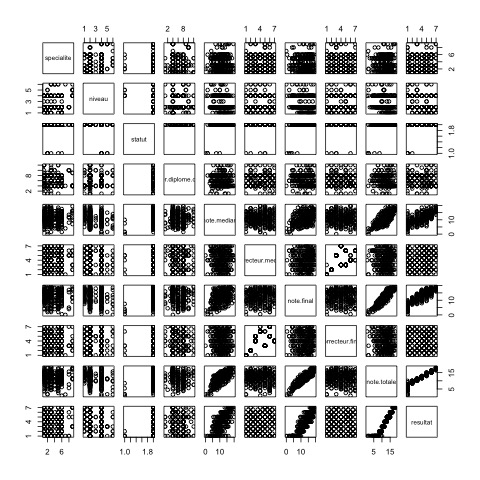
\includegraphics[width=50mm]{Figures/Notes/multiplot.jpg}
	\captionof{figure}{Plot general}
	\label{fig:multiplot_notes}
\end{center}

\subsubsection{Performance et homogénéité}
La figure ci-dessous représente trois diagrammes a boites des notes de médian, final et le résultat de l'UV SY02.
	\begin{center}
			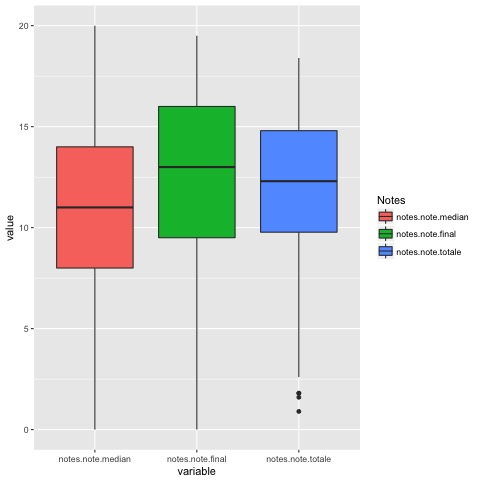
\includegraphics[width=50mm]{Figures/Notes/boxplot_exam.jpg}
			\captionof{figure}{Boxplot des Notes de Median, Final et Totale}
		    \label{fig:Boxplot_notes}
	\end{center}

On remarque que par passage du médian au final les notes ont augmente. En effet ceci est aussi témoigné par le tableau ci-dessous:

\begin{center}
	\begin{tabular}{c c c c c }
		\textbf{Notes} & \textbf{1er Quartl} & \textbf{Medianne}   & \textbf{Moyenne} & \textbf{3em Quartl} \\
		Median  & 8.0 			& 11.0		 & 10.92      & 14.0\\
		Final      & 9.50 		  & 13.0 	   & 12.38	    & 16.0\\
		Totale   & 9.775        & 12.3       &  11.845    & 14.8\\
	\end{tabular}
	\captionof{table}{Notes}
\end{center} 

Il est tout a fait logique que le digramme de résultats se situe entre les 2 puisque que c'est la moyenne \textbf{pondérée??} des 2 notes.
 
	
\subsubsection{Lien entre la réussite, la formation, la branche et le niveau}

	\begin{center}
	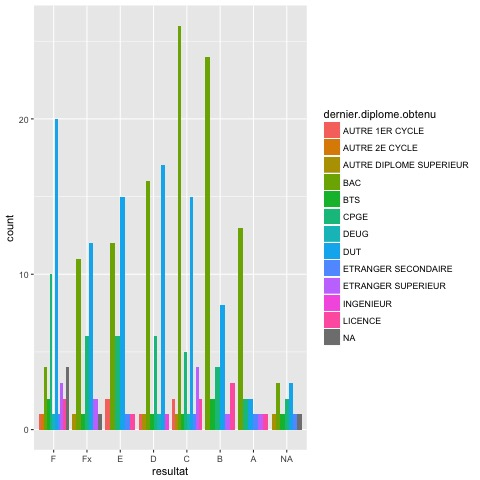
\includegraphics[width=50mm]{Figures/Notes/diplome_resultat.jpg}
	\captionof{figure}{Diagramme a baton de lien entre la formation et le resultat}
	\label{fig:formation_resultat}
	\end{center}



	\begin{center}
	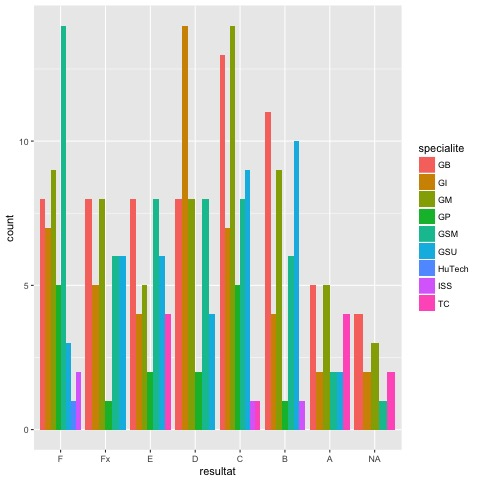
\includegraphics[width=50mm]{Figures/Notes/specialite_resultat.jpg}
	\captionof{figure}{Diagramme a baton de lien entre la branche et le resultat}
	\label{fig:specialite_resultat}
	\end{center}


		\begin{center}
		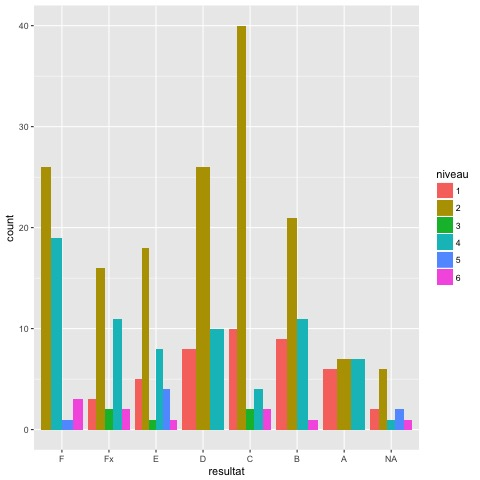
\includegraphics[width=50mm]{Figures/Notes/niveau_resultat.jpg}
		\captionof{figure}{Diagramme a baton de lien entre le niveau et le resultat}
		\label{fig:niveau_resultat}
		\end{center}

\subsubsection{Influence du correcteur sur la note}

	\begin{center}
	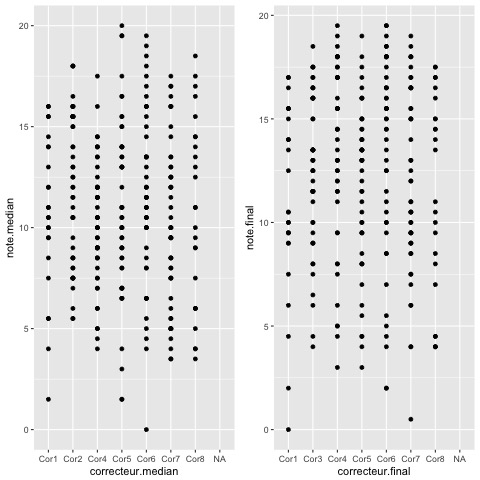
\includegraphics[width=70mm]{Figures/Notes/correcteur.jpg}
	\captionof{figure}{Scatterplot des notes en fonction des correcteurs}
	\label{fig:scatter_correcteur_median}
\end{center}

\section{Conclusion}

\section{Crabs}
Le dataset \textit{"Crabs"} représente un jeu de données de 200 crabes décrits par huit variables, trois sont qualitatives et cinq sont quantitatives.

\subsection{Description des variables}


\begin{itemize}
	\item \textbf{Variables Qualitatives Nominales :}  crabs.sp, crabs. sex, crabs.inde
	\item \textbf{Variables Quantitatives : } crabs.FL, crabs.RW, crabs.CL, crabs.CW, crabs.BD
\end{itemize}

Nous pouvons representer les donnees des variables quantitatives a l'aide un boxplot.
\begin{center}
	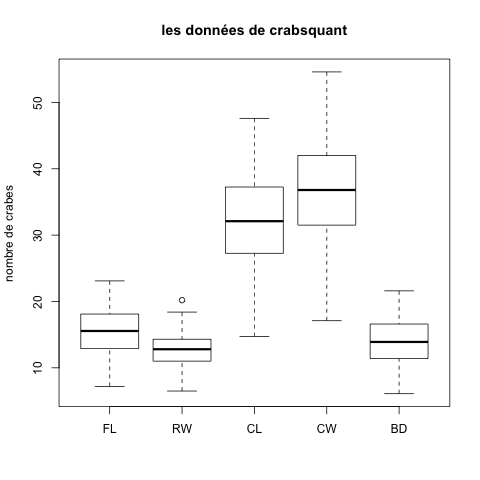
\includegraphics[width=50mm]{Figures/Crabs/bxp_crabsquant.png}
	\captionof{figure}{Boxplot des données quantitaves}
	\label{fig:boxplot_crabs_quantitatives}
\end{center}

Nous remarquons d'ores et deja que deux categories de variables se distinguent, d'un cote FL, RW et BD et d'un autre, CL et CW.

Avant de continuer l'analyse de ces donnees, nous pouvons preciser la signification de chacune de ces variables comme suit:
\begin{itemize}
	\item \textbf{sp:} \textit{(species)}, espece, "B" pour Bleu et "O" pour Orange
	\item \textbf{sex:} sexe, "F" pour Feminin et "M" pour masculin
	\item \textbf{index:} index de 1 a 50 pour chacune des 4 categories suivantes : \{"B,M","O,M","B,F","O,F"\}
	\item \textbf{FL:} Frontal Lobe size en mm
	\item \textbf{RW:} Rear Width en mm
	\item \textbf{CL:} Carapace Length en mm
	\item \textbf{CW:} Carapace Width en mm 
	\item \textbf{BD:} Body Depth en mm
\end{itemize}

\subsection{Analyse descriptive des données}

\subsubsection{Representation de chaque caracteristique en fonction de l'espece}

Afin de voir s'il y a une difference de caracteristiques morphologiques en fonction de l'espece d'abord, nous representons les boites a moustache de chaque variable morphologique en fonction de la variable sp comme suit:

\begin{center}
	\begin{minipage}[t]{0.3\textwidth}
		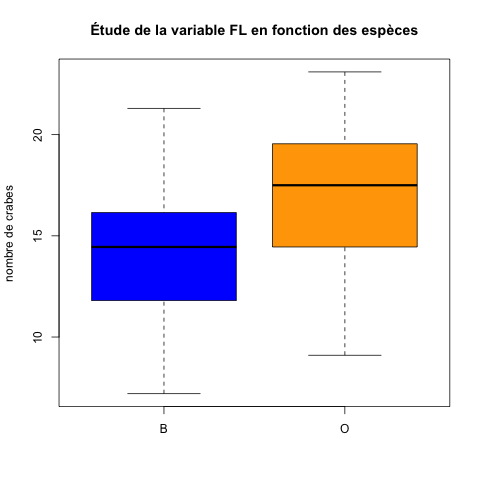
\includegraphics[width=35mm]{Figures/Crabs/bxp_sp_fl.png}
	\end{minipage}
	\begin{minipage}[t]{0.3\textwidth}
		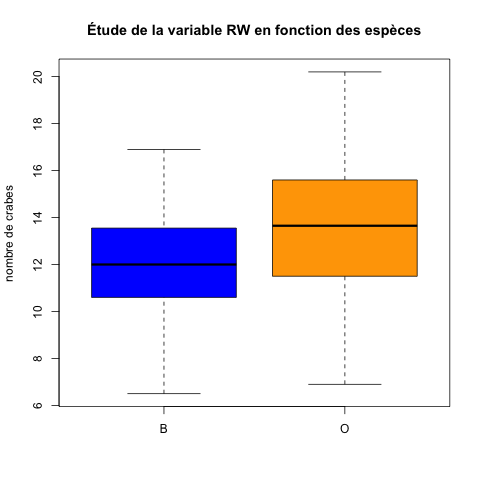
\includegraphics[width=35mm]{Figures/Crabs/bxp_sp_rw.png}	
	\end{minipage}
	\begin{minipage}[t]{0.3\textwidth}
		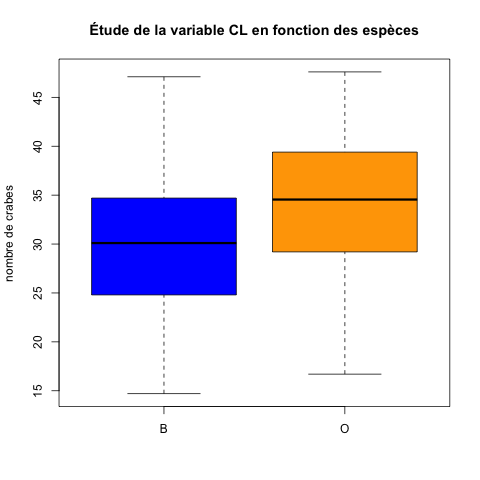
\includegraphics[width=35mm]{Figures/Crabs/bxp_sp_cl.png}
	\end{minipage}
	\newline
	\begin{minipage}[t]{0.3\textwidth}
		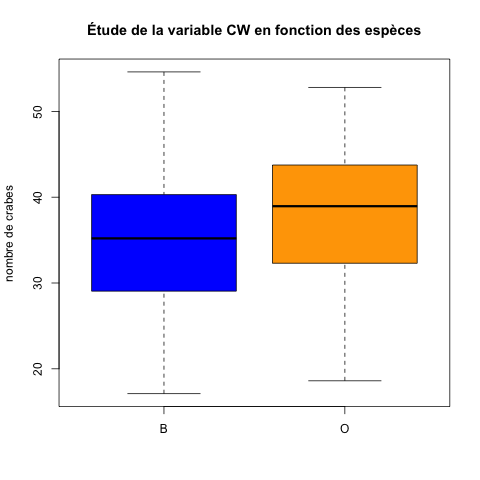
\includegraphics[width=35mm]{Figures/Crabs/bxp_sp_cw.png}	
	\end{minipage}
	\begin{minipage}[t]{0.3\textwidth}
		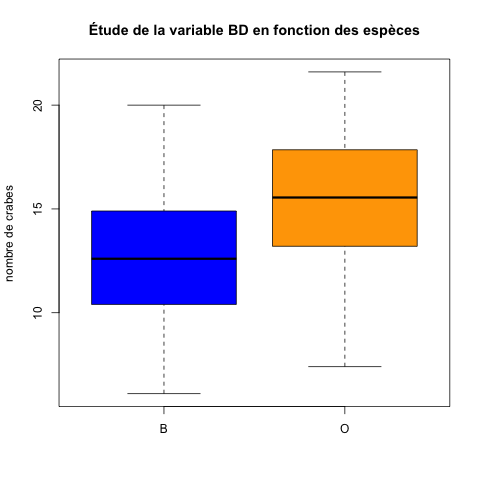
\includegraphics[width=35mm]{Figures/Crabs/bxp_sp_bd.png}
	\end{minipage}
\end{center}

Il y a des distributions assez differentes en fonction de l'espece. Les intervalles de confiances ne se chevauchent pas . Cependant, la dispersion des donnees reste assez homogene au vue des boxplots.
\subsubsection{Representation de chaque caracteristique en fonction du sexe}

Afin de voir s'il y a une difference de caracteristiques morphologiques en fonction du sexe, nous representons les boites a moustache de chaque variable morphologique en fonction de la variable sex comme suit:

\begin{center}
	\begin{minipage}[t]{0.3\textwidth}
		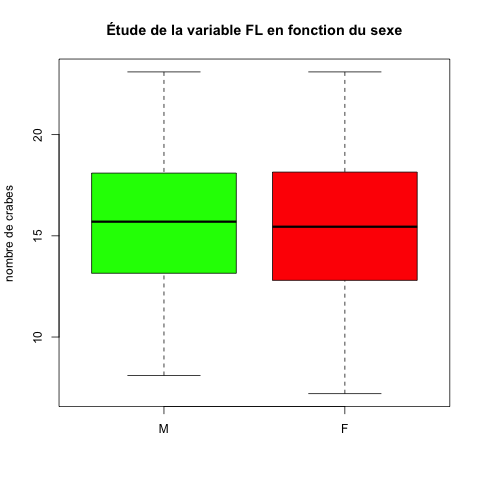
\includegraphics[width=35mm]{Figures/Crabs/bxp_sex_fl.png}
	\end{minipage}
	\begin{minipage}[t]{0.3\textwidth}
		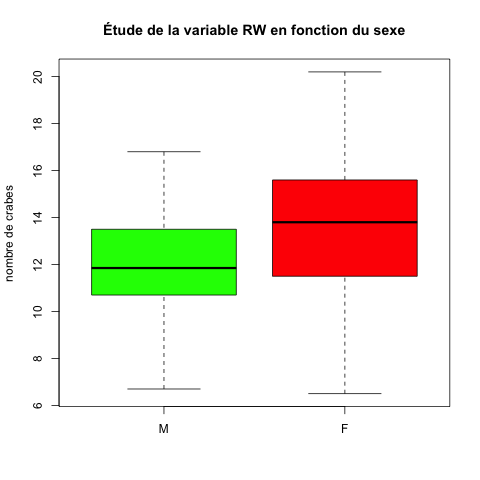
\includegraphics[width=35mm]{Figures/Crabs/bxp_sex_rw.png}	
	\end{minipage}
	\begin{minipage}[t]{0.3\textwidth}
		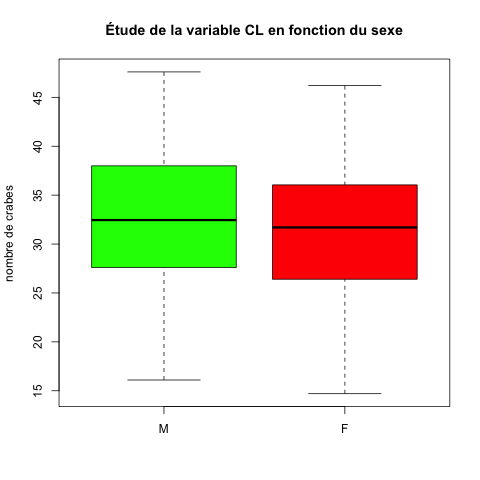
\includegraphics[width=35mm]{Figures/Crabs/bxp_sex_cl.png}
	\end{minipage}
	\newline
	\begin{minipage}[t]{0.4\textwidth}
		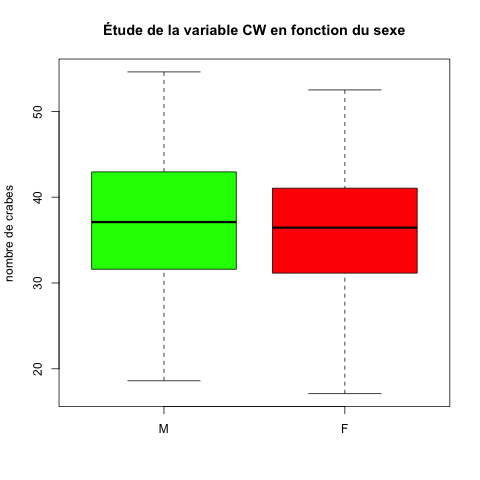
\includegraphics[width=35mm]{Figures/Crabs/bxp_sex_cw.png}	
	\end{minipage}
	\begin{minipage}[t]{0.4\textwidth}
		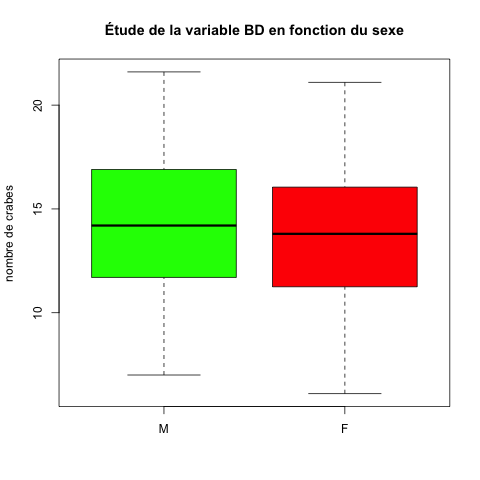
\includegraphics[width=35mm]{Figures/Crabs/bxp_sex_bd.png}
	\end{minipage}
\end{center}

A l'oppose des boxplot en fonction de l'espece, ceux en fonction du sexe relevent une similitude de la distribution des differentes caracteristiques pour la plupart, ainsi que la dispersion des donnees. Nos observons que la variable RW se distingue des autres avec un largeur de l'arriere importante chez les femmes que chez les hommes.

Enfin, la nature de l'espece impacte les caracteristiques morphologiques, a la difference du sexe, qui lui n'influe que peu ces caracteristiques.
\subsubsection{Lien entre les variables}
\begin{center}
	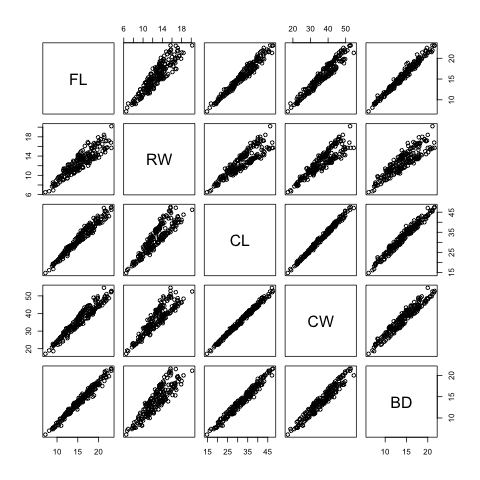
\includegraphics[width=50mm]{Figures/Crabs/plot_crabsquant.png}
	\captionof{figure}{Plot general}
	\label{fig:multiplot_crabs}
\end{center}

Nous pouvons representer chacune de ces variables quantitatives en fonction de l'espece puis en fonction du sexe afin de determiner la possibilite d'identifier l'une ou l'autre a partir des caracteristiques morphologiques. \\

\begin{minipage}[t]{0.6\textwidth}
	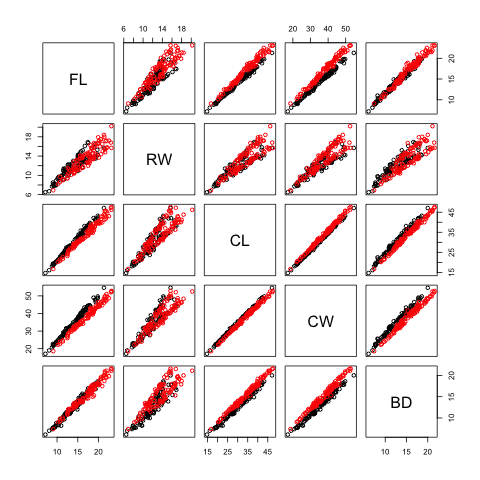
\includegraphics[width=50mm]{Figures/Crabs/plot_crabsquant_sp.png}
\end{minipage}
\begin{minipage}[t]{0.6\textwidth}
	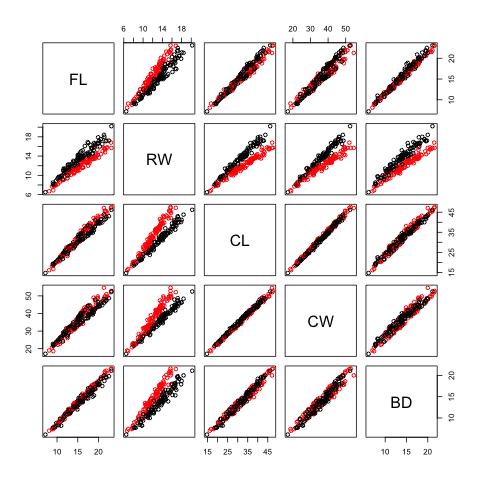
\includegraphics[width=50mm]{Figures/Crabs/plot_crabsquant_sex.png}	
\end{minipage}
\begin{center}
	\captionof{figure}{Plot general en fonction de l'espece (gauche) et du sexe(droite)}
	\label{fig:multiplot_crabs__sp_sex}
\end{center}

Nous remarquons que ni l'espece ni le sexe ne peuvent vraiment etre identifies a partir d'une ou de plusieurs caracteristiques morphologiques.
En effet, dans les cas, l'ensemble des points est represente sur une meme droite, on ne peut pas clairement distinguer l'une difference. De ce fait, il est difficile de reconnaitre une espece selon ses carateristiques morphologiques.

\subsection{Analyse de la correlation}

\begin{center}
	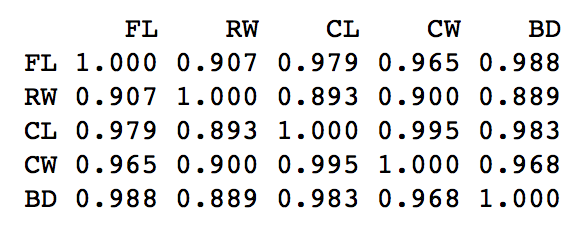
\includegraphics[width=50mm]{Figures/Crabs/cor_crabsquant.png}
	\captionof{figure}{Correlation entre les variables}
	\label{fig:cor_carbsquant}
\end{center}

Il y a une forte correlation positive entre toutes les combinaisons de variables, telle que la valeur minimale observee est 0.889. 
Il s'agit de la taille des membres du corps d'un crabe, il semble donc logique et naturel qu'elles soient proportionnelles entre elles.
Une des facons pour s'affranchir de ce phenomene est de diviser chaque valeur par la somme totale de toutes celles de l'individu.

\section{Pima}
Le dataset \textit{"Pima"} représente un jeu de données constitue de 532 individus tous de sexe feminin décrits par huit variables dont une qualitative et sept sont quantitatives.

\subsection{Description des variables}


\begin{itemize}
	\item \textbf{Variables Qualitatives Ordinale :}  Pima.z
	\item \textbf{Variables Quantitatives : } Pima.npreg, Pima.glu, Pima.bp, Pima.skin, Pima.bmi, Pima.ped, Pima.age
\end{itemize}

Nous pouvons representer les donnees des variables quantitatives a l'aide un boxplot.
\begin{center}
	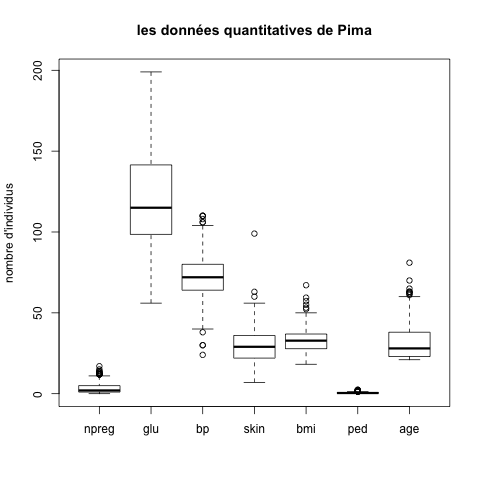
\includegraphics[width=50mm]{Figures/Pima/bxp_Pimaquant.png}
	\captionof{figure}{Boxplot des données quantitaves}
	\label{fig:boxplot_pima_quantitatives}
\end{center}

\subsection{Analyse descriptive des données}

\subsubsection{Representation de chaque caracteristique en fonction de z (diabetique ou pas)}

\begin{center}
	\begin{minipage}[t]{0.3\textwidth}
		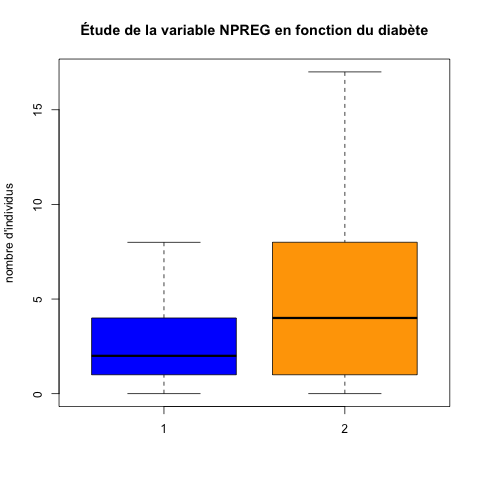
\includegraphics[width=35mm]{Figures/Pima/bxp_z_npreg.png}
	\end{minipage}
	\begin{minipage}[t]{0.3\textwidth}
		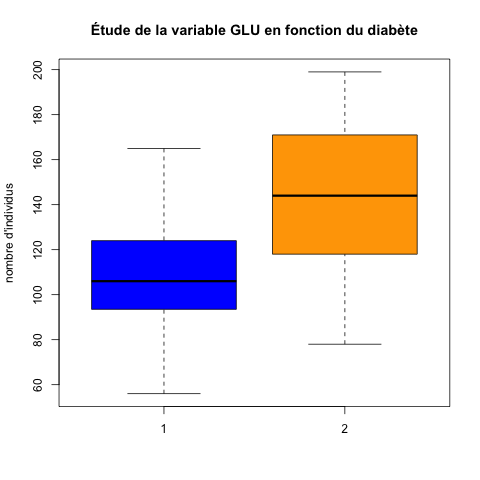
\includegraphics[width=35mm]{Figures/Pima/bxp_z_glu.png}	
	\end{minipage}
	\begin{minipage}[t]{0.3\textwidth}
		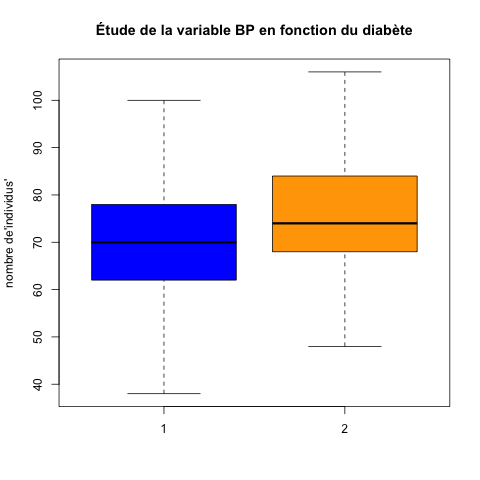
\includegraphics[width=35mm]{Figures/Pima/bxp_z_bp.png}
	\end{minipage}
	\newline
	\begin{minipage}[t]{0.3\textwidth}
		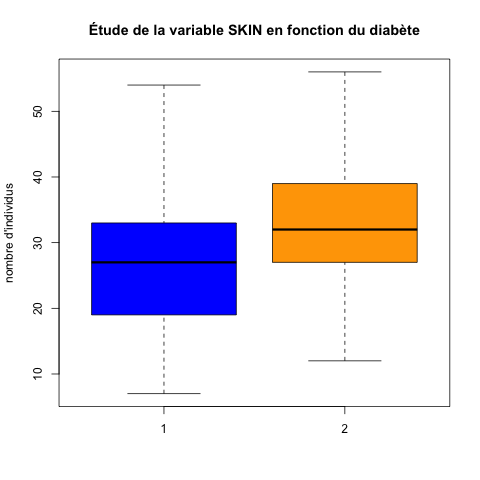
\includegraphics[width=35mm]{Figures/Pima/bxp_z_skin.png}	
	\end{minipage}
	\begin{minipage}[t]{0.3\textwidth}
		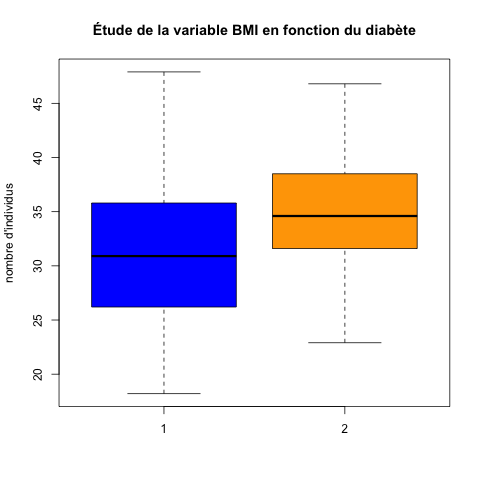
\includegraphics[width=35mm]{Figures/Pima/bxp_z_bmi.png}
	\end{minipage}
	\newline
	\begin{minipage}[t]{0.3\textwidth}
		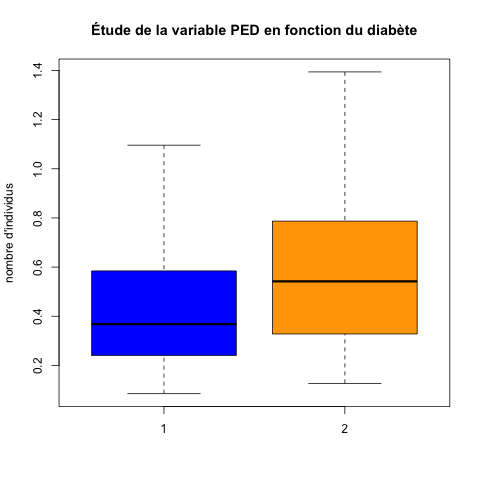
\includegraphics[width=35mm]{Figures/Pima/bxp_z_ped.png}
	\end{minipage}
	\begin{minipage}[t]{0.3\textwidth}
		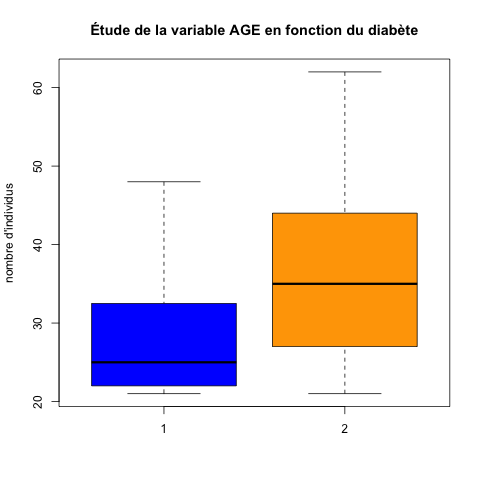
\includegraphics[width=35mm]{Figures/Pima/bxp_z_age.png}
	\end{minipage}
\end{center}

\subsubsection{Lien entre les variables}


\chapter{Analyse Composantes Principales}
\end{document}
